%%% Copyright (C) 2004 Claire M. Connelly and 
%%% the Department of Mathematics, Harvey Mudd College.
%%%
%%% This file is part of the sample thesis document provided to HMC
%%% mathematics students.
%%%
%%% See the COPYING document, which should accompany this
%%% distribution, for information about distribution and modification
%%% of the document and its components.

\chapter{Automation of PilotCity Programming}%
\label{sec:mathematical-notation}

\subsection{Background}
This project requires consideration of high level social problems related to education, including an analysis of the effectiveness of Project Based Learning versus Work Based Learning. It also includes analyzing more standard technical problems such as matching PilotCity users, and building out a platform with which these users can interact. The various challenges in this project combine into a unique problem space involving the analysis of uncurated data for educational advancement.

At the start of this project, we had limited access to historic user data from PilotCity. We conducted a series of user interviews to incorporate feedback into the construction of a recommender system. We interviewed students, teachers, employers, and school district administrators to gather information regarding pain points of PilotCity's past programming, the value of Project Based Learning, and ideas for an online platform for PilotCity. We compiled interview notes and accordingly planned a web application that can onboard and recommend matches between employers and classrooms. 

\subsection{Web Interface For PilotCity Users}

	Our initial technical work involved creating the front-end onboarding platform to start building the web application. We created a sequence of pages in which teachers and employers could fill in relevant information that allowed us to make the most optimal recommendations. Once we had a functional front-end product, we handed off the front-end work to PilotCity's local team. Figures \ref{fig:usertype}-\ref{fig:completed} demonstrate the front-end flow built by the team, as viewed by an onboarding teacher.
	
    \begin{figure}[H]
        \centering
        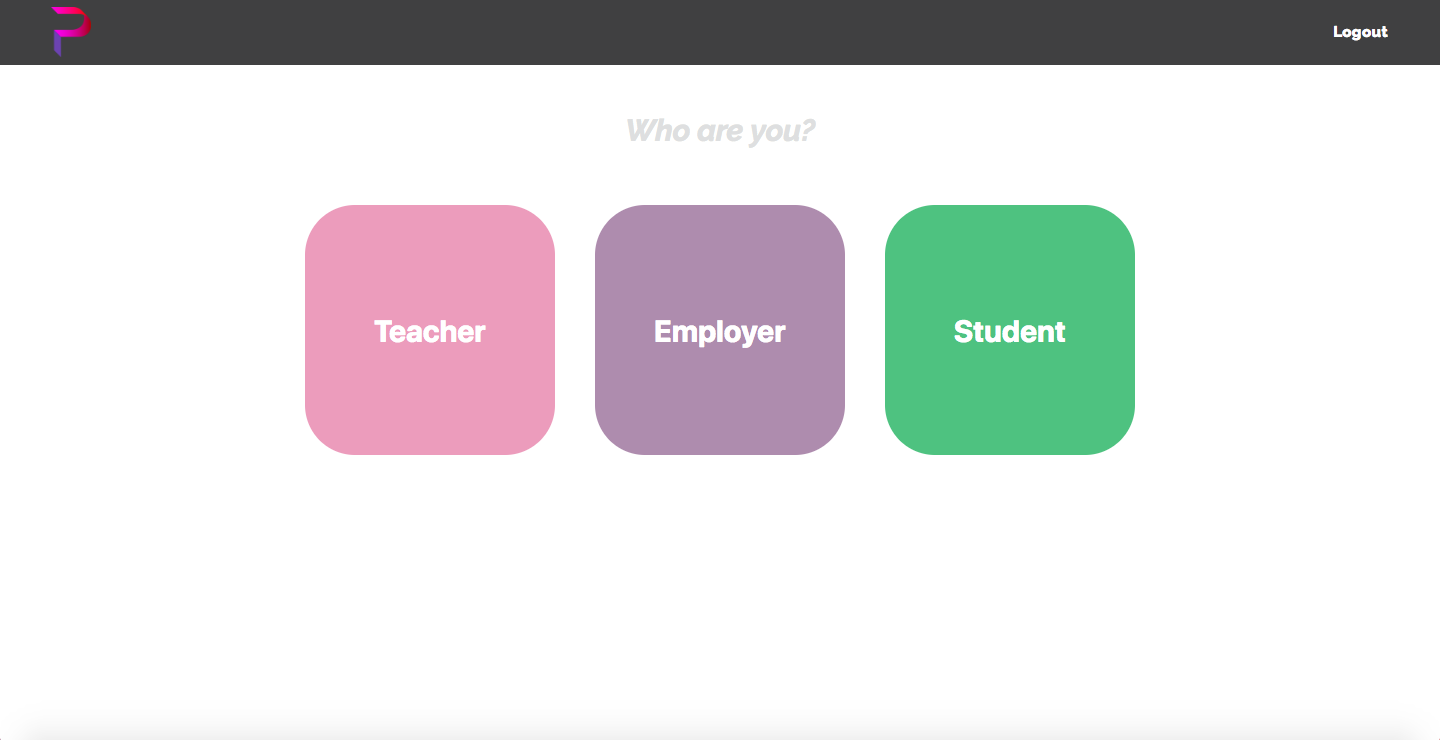
\includegraphics[scale=0.2]{type.png}
        \caption{Front-end view of what the user sees when beginning their PilotCity onboarding process. The user would then proceed accordingly, specifying what user category they would fall into.}
        \label{fig:usertype}
    \end{figure}

    \begin{figure}[H]
        \centering
        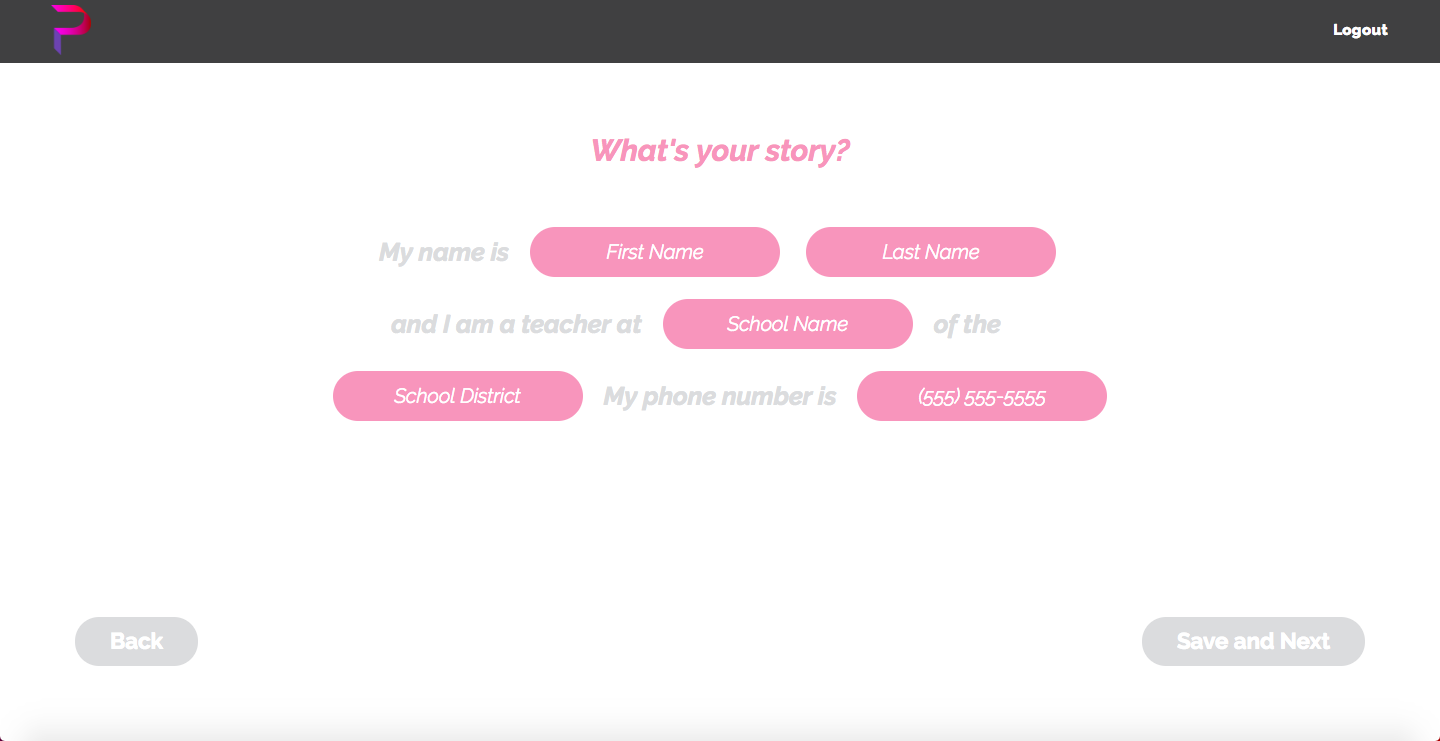
\includegraphics[scale=0.2]{story.png}
        \caption{The next page seen by an onboarding teacher. Here, the teacher is asked about the school they teach at and their contact information.}
        \label{fig:whatsurstory}
    \end{figure}
    
    \begin{figure}[H]
        \centering
        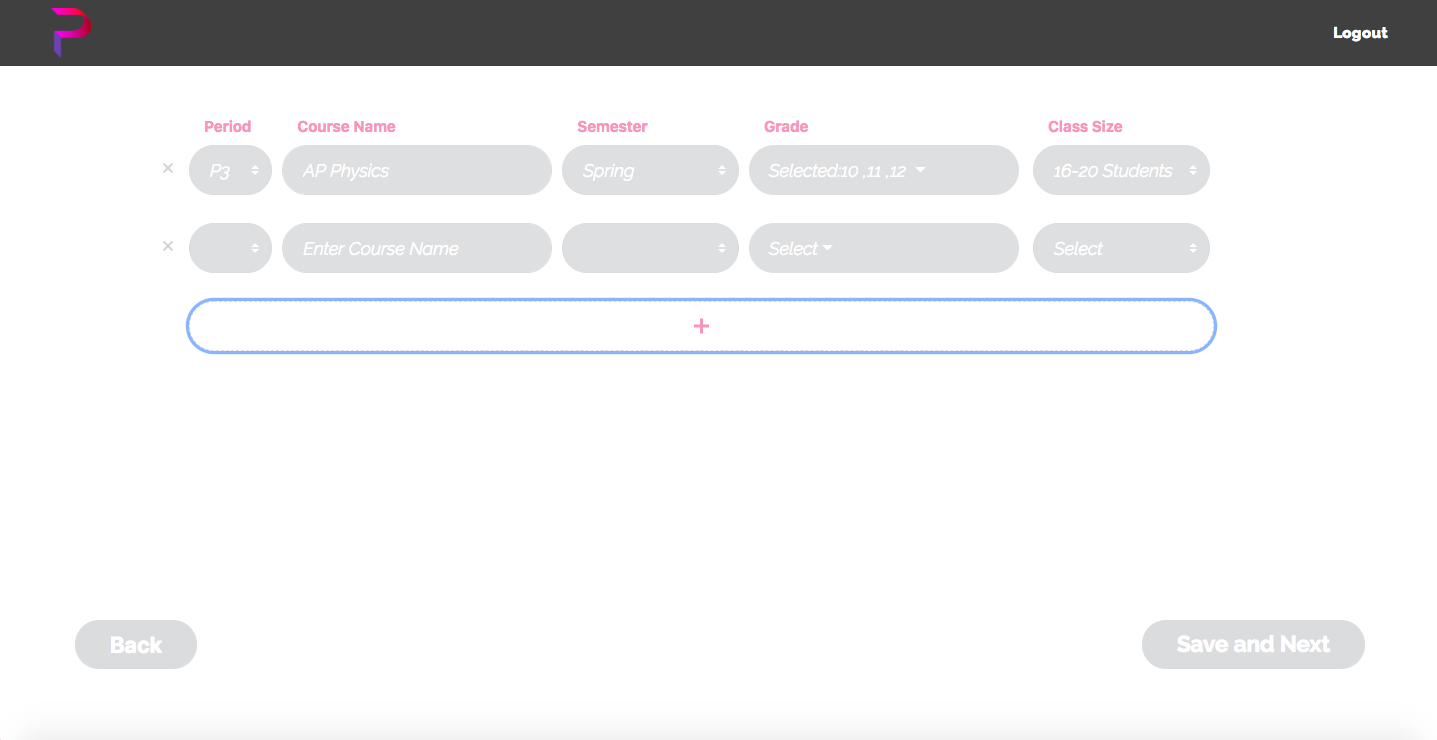
\includegraphics[scale=0.2]{classroom.png}
        \caption{Front-end view where the onboarding teacher is asked about the classes they want to involve in the PilotCity program.}
        \label{fig:describeclassroom}
    \end{figure}
    
    \begin{figure}[H]
        \centering
        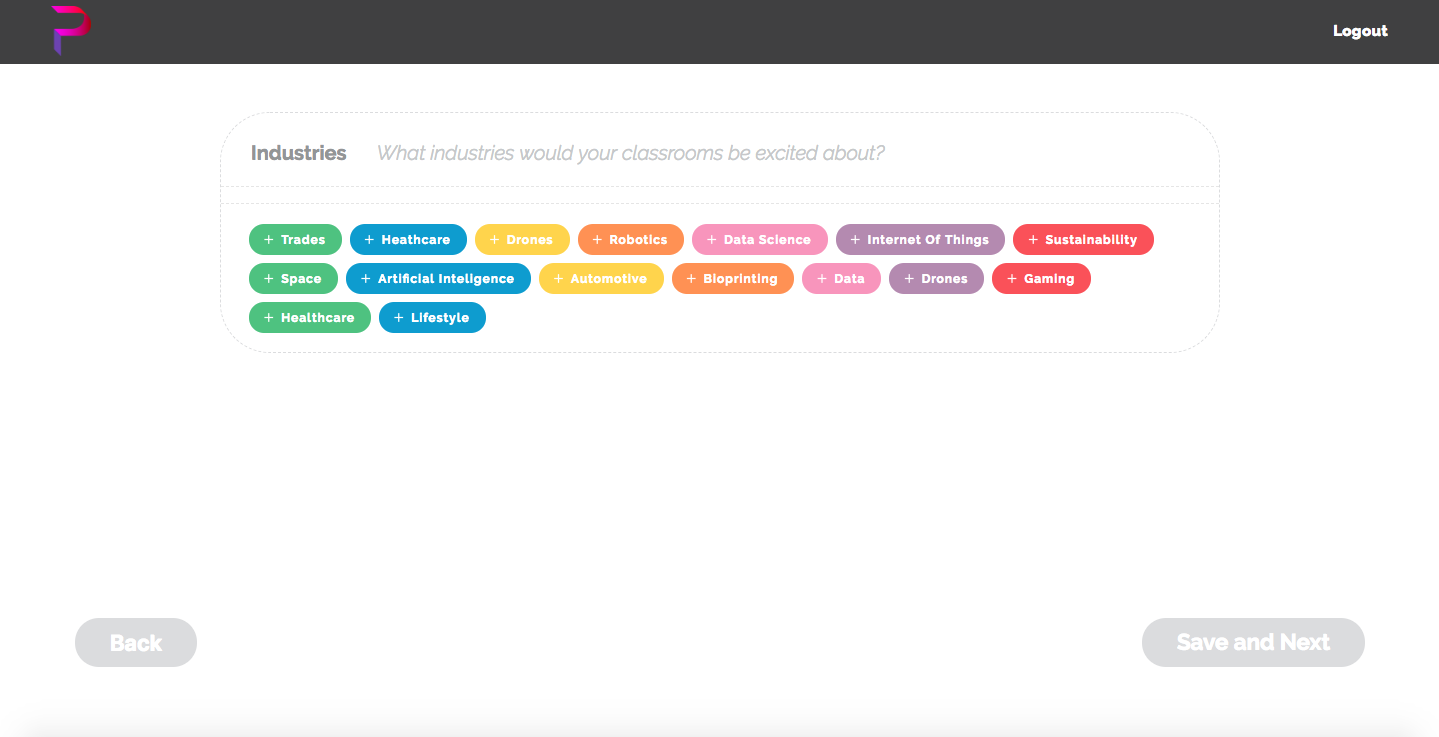
\includegraphics[scale=0.2]{industry.png}
        \caption{Front-end view where the onboarding teacher is asked about the industries that their classrooms would be interested in working with.}
        \label{fig:industrypref}
    \end{figure}
    
    \begin{figure}[H]
        \centering
        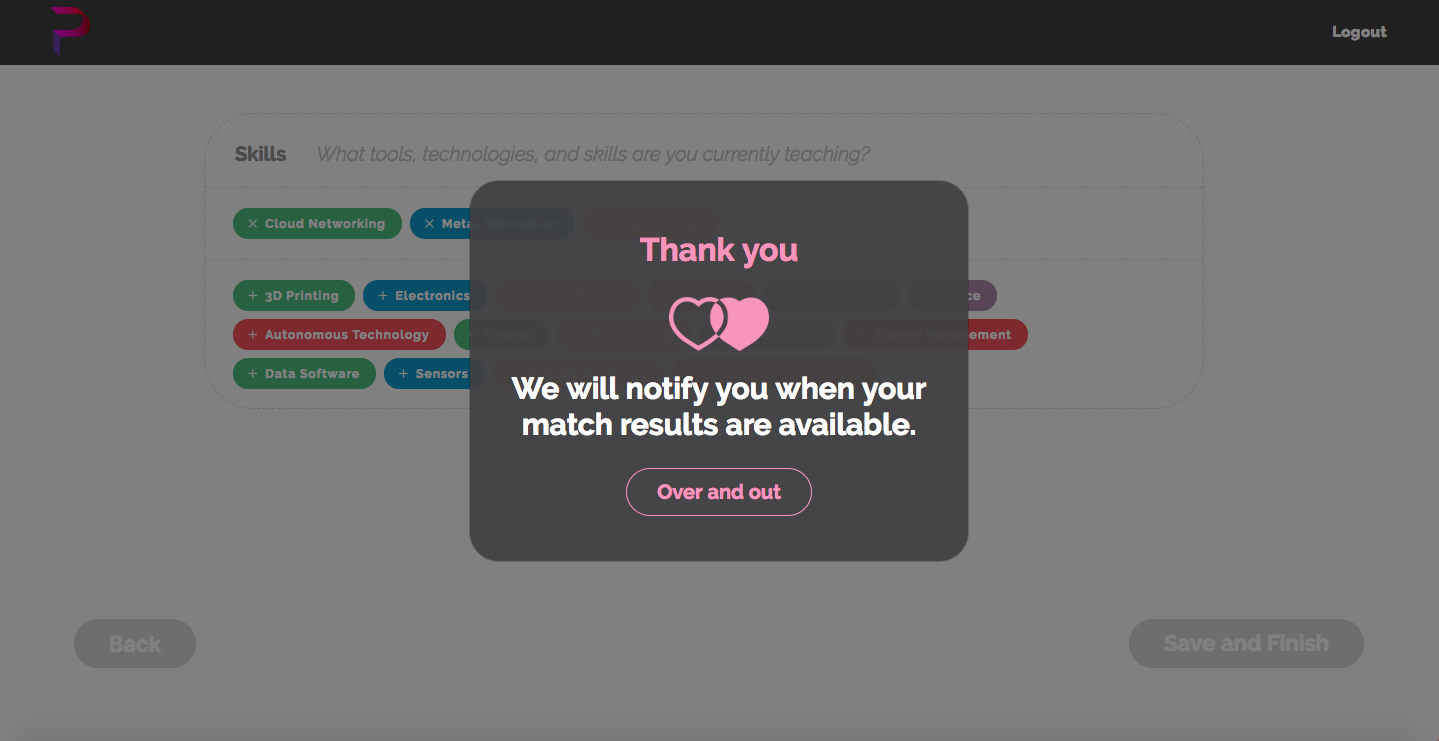
\includegraphics[scale=0.2]{end.png}
        \caption{View that the teacher would see once finishing the onboarding process. This page indicates to the user that their information has been saved, and that they will be contacted as soon as employer recommendations are available for each of their classrooms.}
        \label{fig:completed}
    \end{figure}

\subsection{Recommender System}

	We planned and implemented a recommender system to recommend classrooms to employers and employers to teachers based on similarities in industry and skills. We score classrooms for an employer and employers for a teacher using the GloVe Model, which represents words as vectors capturing semantic meaning. The similarity score between two words is taken to be the cosine of the angle between the vector representation of the two words. We further adapt the GloVe model's output to be able to take in two phrases with multiple words, such as "Machine Learning" and "Artificial Intelligence" and compute their similarity. This is done by taking the average of each pairwise similarity between individual words.
	
	The final score between an employer and a classroom is a weighted combination of the similarity scores between the inputs of employers and teachers. For each employer, we consider their industry, service, product, their vision for working with high school students, and the location of their workplace. For each classroom, we consider the course name, the industry preference of the teacher, the tools, technologies, and skills taught in the classroom, and the location of the school. The UI of the final recommendation system, as viewed by a logged in employer, is shown in figure \ref{fig:recommender_system} below. The final recommender system was meant to serve as a baseline ordering from which teachers and employers could easily choose suitable matches. 
	
	\begin{figure}[H]
        \centering
        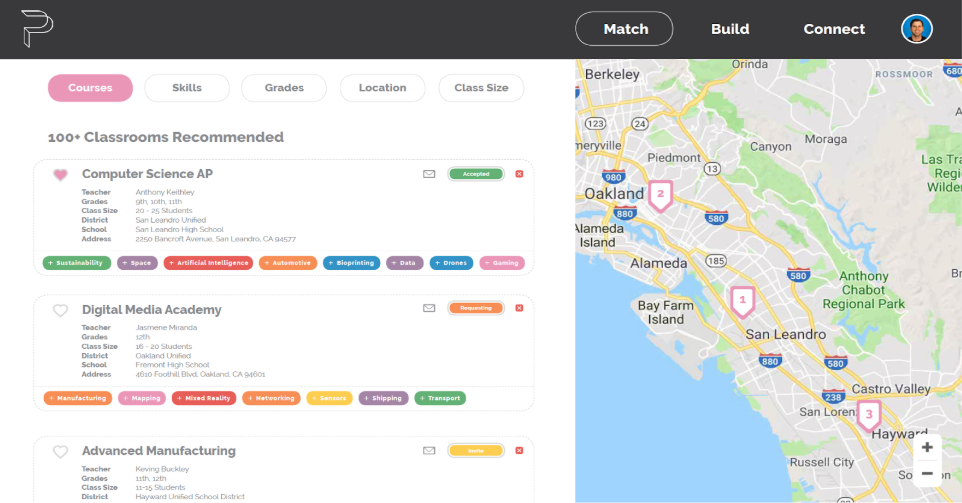
\includegraphics[scale=0.35]{recommender_ui.png}
        \caption{UI for the Recommender system}
        \label{fig:recommender_system}
    \end{figure}
	
\subsection{Evaluation of Recommender System}

The recommender system, due to a miscommunication between ourselves and the local team, was not correctly incorporated into PilotCity's website at the time of project placement which occurred over our winter break. For this reason, PilotCity made the final matches as they had done in previous years. We then evaluated our recommender system against the final project-placements in the following way. For each employer's assigned classrooms, we recorded what rank our recommender system gave each classroom. For example, one employer, the City of Hayward, was assigned 7 classrooms for spring 2019. Our recommender gave these 7 classrooms the ranks shown in the "our ranks" row in table \ref{tab:comp} below. We compare these ranks to what the "ideal ranks" would be (also shown table \ref{tab:comp}). Note that the lower the number, the more highly it is ranked (the classroom given a rank of 0 is the most highly-recommended classroom).

\begin{table}[H]
\begin{center}
\begin{tabular}{|l|l|l|l|l|l|l|l|l|l|l|l|l|l|l|}
\hline
\textbf{classroom}   & A  & B  & C  & D   & E & F & G  \\
\hline
\textbf{our ranks}   &  13 & 16 & 14 & 15 & 30 & 91 & 29  \\
\hline
\textbf{ideal ranks} & 0  & 1  & 2   & 3   & 4 & 5 & 6   \\
\hline
\end{tabular}
\end{center}
\caption{Comparison of classroom ranks for City of Hayward}
\label{tab:comp}
\end{table}


We can see from table \ref{tab:comp} above that our recommender, though imperfect, ranked the majority of the classrooms relatively high (13th, 14th, 15th, 16th place), yet some of the classrooms were ranked much deeper down the list, especially the outlier in 91st place. We create a score to encapsulate this trend.

Since all of the classrooms placed with the City of Hayward are equally suitable placements, any permutation of the ideal ranks is equally ideal. In order to account for this, our metric takes the median of our rank and compares that to the median of the ideal rank. We then subtract the median of the ideal rank from the median of our algorithm's rank to get a sense of how well, in aggregate, our recommender did for a given employer relative to that employer's ideal matching. For the above example with the City of Hayward, the score comes out to: 

$$ median(our\ ranks) - median(ideal\ ranks) = 16 - 3 = 13$$

Using the scoring method just described and averaging across all employers, our recommender system got a score of 34. Relative to over 150 total classrooms, this score is expected. Many of the variables that informed the final employer-classroom pairing decisions were factors we were advised to ignore to simplify the onboarding process, such as schedule and availability.

We considered tuning our recommender system's algorithm to minimize the score described above. However, we agree that at this stage with only 35 employers this approach would probably overfit our algorithm, especially as our score currently makes the strong assumption that each employer's "ideal" classrooms were the ones to which they were assigned. A more informative approach would be to gather data about how well classrooms and employers enjoyed their partnership and incorporate this into future recommender system iterations.

\subsection{Impact}

	A primary goal of our project has been to improve scalability, automation, and user engagement of PilotCity's efforts. 
	PilotCity having a website this year led to a major influx of new users. As PilotCity grows, they will be able to build off of our recommendation tool to optimize for the most successful classroom-employer partnerships. These improvements to PilotCity's programming may allow for more connections between high school students and workplace opportunities. These educational opportunities and general local connections benefit countless students and local cities which PilotCity serves. 

\subsection{Code}
    Our code is available on github.com/hmcmathclinic/18-19-PilotCity-Code and the most current version of the website can be viewed at pilotcity.com. 
